\section{Experimental results}

%\paragraph{Task/Problem.}
As many real-world datasets contain missing values, missing data imputation has been a popular problem to tackle in statistics and machine learning~\cite{little1986statistical, nelwamondo2007missing}.
GNNs have recently proved to be a powerful tool for this task~\cite{spinelli2020neural}.
With a view that our method incorporates additional higher-dimensional structure in the data, we evaluate the performance of the SNNs in imputing missing data over simplicial complexes.

\paragraph{Data.}
A \emph{coauthorship complex}~\cite{patania2017} is a simplicial complex where a paper with $k$ authors is represented by a $(k-1)$-simplex (see Figure~\ref{fig:data2complex} and the supplementary material for detailed definitions). The added subsimplices of the $k-1$-simplex are interpreted as collaborations among subgroups of authors.
We sampled two coauthorship complexes---CC1 and CC2, see Table~\ref{table:Simplices-coauthor} for statistics---from the Semantic Scholar Open Research Corpus~\cite{ammar18NAACL}, a dataset of over $39$ million research papers with authors and citations\footnote{Papers with fewer than $5$ citations or more than $10$ authors were excluded.}.
We believe the following procedure extracts representative papers from which one can construct coauthorship complexes: We performed random walks (of length $80$) on the vertices of the graph which correspond to papers, and edges connect papers sharing at least one author. The $k$-cochains are given by the number of shared citations of the given collaboration (see Figure~\ref{fig:data2complex} and~\ref{fig:bipartite}(b)-(c)).
\paragraph{Method.}
We evaluated the performance of the SNNs on the task of imputing missing data on the $k$-cochains (for $k=0,1,2$) of the extracted coauthorship complexes. As in a typical pipeline for this task~\cite{nelwamondo2007missing}, missing data is artificially introduced by replacing a portion of the values with a constant. Specifically, given a fixed coauthorship complex, missing data is introduced at random on the $k$-cochains at $4$ rates: $10\%,  20\%,  30\%$, and $50\%$. The training input is then given by the $k$-cochains on which the random missing data is substituted by the median of the known data (the median is perhaps a reasonable first guess for estimating missing data). We trained an SNN comprising $3$ layers with $30$ convolutional filters of degree $5$. We used the $L_1$ norm as the reconstruction loss over the known elements, and the Adam optimizer with a learning rate of $10^{-3}$. The SNN was trained for $1000$ iterations. We then tested the performance of the network on its accuracy in imputing missing data. As a statistical evaluation, we tested the network on different random samples of the damaged portions for the same percentage of missing value.
\paragraph{Results.}
Figure~\ref{fig:accuracy-error} (a-b) shows the mean accuracy (MA) and absolute error distribution (AED) (see the supplementary material for definitions) of the SNN in inputing missing citations on CC1. Observe that the distribution of the prediction error accumulates close to zero.

\begin{figure}[tb]
\centering
 \begin{subfigure}[t]{-0.8\textwidth}
 \vspace{-4cm}
    \text{(a)}
  \end{subfigure}
\begin{subfigure}[t]{0.8\textwidth}
\centering
   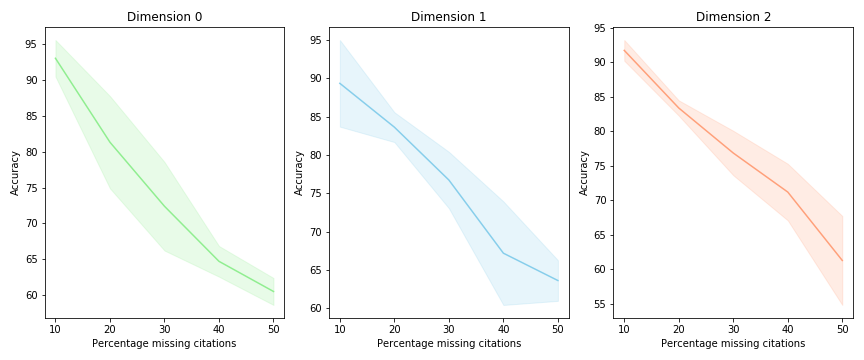
\includegraphics[scale=0.35]{./figures/accuracy_network1.png}
\end{subfigure}
 \begin{subfigure}[t]{0.8\textwidth}
    \text{(b)}
  \end{subfigure}
\begin{subfigure}[t]{0.8\textwidth}
\centering
\vspace{-0.5cm}
   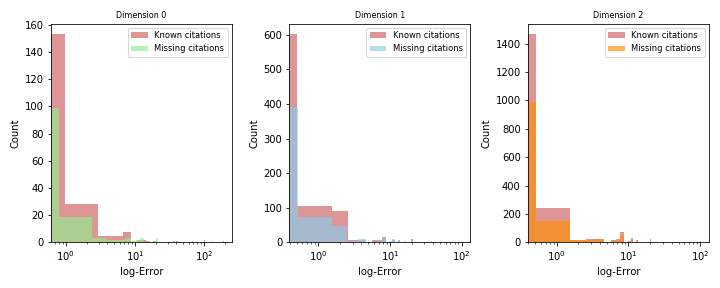
\includegraphics[scale=0.36]{./figures/Error_dist_start150250_seed6666_notsee40.png}
\end{subfigure}
\caption{(a) Mean Accuracy $\pm$ standard deviation over 5 samples of SNN in imputing missing citations on CC1. (b) Absolute Error Distribution over 1 sample for $40\%$ missing values in CC1.}
\label{fig:accuracy-error}
\end{figure}


As a second assessment, we evaluate how accurately an SNN trained on one coauthorship complex can impute missing citations on a different complex. Over the assumption that coauthorship complexes share a similar structure and the same data underlies the generating process of cochains.
Figure~\ref{fig:transfer-learning} shows the MA in predicting missing citations on CC1 using the above architecture of SNN trained on CC2. Observe that the accuracy of the pretrained network on CC2 is comparable to the result shown in Figure~\ref{fig:accuracy-error}. We believe that this is expected in situations where the topological structure of the underlying complex is similar before and after transfer.

Table~\ref{table:comparison-SNN} shows the performance of two baselines: missing values inferred as (i) the mean or median of all known values, and (ii) the mean of the $(k-1)$ and $(k+1)$ neighboring simplices.
SNNs well outperform these baselines.
Comparison with stronger imputation algorithms is left for future work.

\begin{figure}[htbp]
  \centering
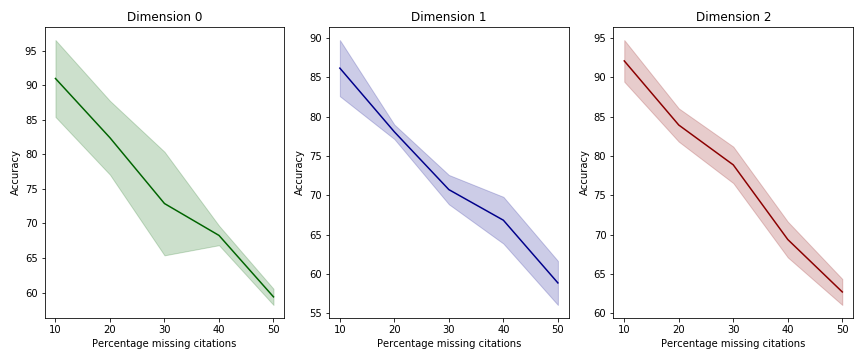
\includegraphics[scale=0.35]{./figures/accuracy_network1_pretrained.png}
  \caption{Mean Accuracy $\pm$ standard deviation over 5 samples in imputing missing citations on CC1 with an SNN trained on CC2.} \label{fig:transfer-learning}
\end{figure}

\begin{table}[htbp]
  \centering
  \scriptsize{
  \begin{tabular}{lrrrrrr}
    \toprule
    Method   & CC1 - dim 0   & CC1 - dim 1   & CC1 - dim 2   & CC2 - dim 0  & CC2 - dim 1  & CC2 - dim 2 \\
    \midrule
    Global Mean & $3.30 \pm 0.82$ & $5.75\pm 1.28$  &$ 2.96\pm 0.49$  & $3.32 \pm 0.85$ & $8.31 \pm 1.03$  & $7.90\pm 0.35$\\
    Global Median & $7.78 \pm 2.70$   & $10.44 \pm 1.00$ &$ 12.50 \pm 0.63 $ & $5.55 \pm 0.38 $&$ 6.28\pm 0.36  $&$ 6.06\pm 0.20$\\
    Neighbors Mean & $11.88\pm 5.29 $& $24.15 \pm 1.85$ & $27.38 \pm 1.18  $& $16.45 \pm 1.83 $&$ 30.67\pm 2.13$   &$ 24.85 \pm 0.57 $\\
    \bottomrule
  \end{tabular}}
  \vspace{2pt}
  \caption{%
      Performance of baselines: Mean Accuracy $\pm$ standard deviation for $30\%$ missing data over 5 samples.
  }\label{table:comparison-SNN}
\end{table}
